% CENG 467 — Dönem Projesi Sunumu
% Controllable Text Generation via Diffusion Models
% Süre: 15 dk | Tema: Madrid | Dil: Türkçe | Hedef: sınıf arkadaşları
%
% Build: tectonic presentation.tex

\documentclass[10pt,aspectratio=169]{beamer}

\usetheme{Madrid}
\usecolortheme{default}

% Tectonic = XeTeX → UTF-8 native, fontspec ile lmodern OTF dosya isimleri
\usepackage{fontspec}
\setmainfont{lmroman10-regular}[
  Extension=.otf,
  BoldFont=lmroman10-bold,
  ItalicFont=lmroman10-italic,
  BoldItalicFont=lmroman10-bolditalic]
\setsansfont{lmsans10-regular}[
  Extension=.otf,
  BoldFont=lmsans10-bold,
  ItalicFont=lmsans10-oblique,
  BoldItalicFont=lmsans10-boldoblique]
\setmonofont{lmmono10-regular}[
  Extension=.otf,
  BoldFont=lmmonolt10-bold,
  ItalicFont=lmmono10-italic]
\usepackage[shorthands=off,turkish]{babel}
\usepackage{microtype}
\usepackage{booktabs}
\usepackage{amsmath,amssymb}
\usepackage{tikz}
\usepackage{xcolor}

\setbeamertemplate{navigation symbols}{}
\setbeamerfont{footline}{size=\tiny}

\title[Diffusion-LM \\ E2E NLG]{Diffusion Modelleri ile Kontrol Edilebilir Metin Üretimi}
\subtitle{Görüntülerden tanıdığımız yöntemi metne taşımak}
\author[Z. Almaho]{Zübeyr Almaho \\ \small (300201023)}
\institute[İYTE]{İzmir Yüksek Teknoloji Enstitüsü \\ Bilgisayar Mühendisliği Bölümü \\
\vspace{0.3em}\footnotesize CENG 467 --- Doğal Dil Anlama ve Üretme \\
Öğretim Üyesi: Prof.\ Dr.\ Aytuğ Onan}
\date{Bahar 2026}

\begin{document}

%==============================================================================
\begin{frame}
  \titlepage
\end{frame}

%==============================================================================
\begin{frame}{Sunum Akışı}
  \begin{enumerate}
    \item Hangi projeyi seçtim ve neden ilginç buldum?
    \item Görev: E2E NLG --- restoran açıklamaları üretmek
    \item Diffusion modeli nedir? (sezgisel anlatım)
    \item Diffusion-LM nasıl çalışıyor? (adım adım)
    \item Geliştirirken neyle karşılaştım? --- gerçek hatalar, çözümler
    \item Sonuçlar ve karşılaştırma
    \item Ne öğrendim?
  \end{enumerate}
\end{frame}

%==============================================================================
\section{Projenin hikâyesi}

\begin{frame}{Hangi projeyi seçtim?}
  \begin{block}{Konu \#4 --- Controllable Text Generation via Diffusion Models}
    Hocanın listesinden bu konuyu seçmemin sebebi:
    \begin{itemize}
      \item Görüntü üretiminde \textbf{diffusion} herkesin bildiği bir şey
            (Stable Diffusion, DALL·E, Midjourney)
      \item Aynı fikrin \textbf{metne} uygulanması hâlâ aktif bir araştırma alanı
      \item ChatGPT/GPT-4 gibi otoregresif modellerin alternatifi:
            \emph{farklı bir paradigma}
    \end{itemize}
  \end{block}

  \begin{exampleblock}{Aklımdaki soru}
    Görüntüde bu kadar iyi çalışan bir yöntem, metinde nasıl çalışır?
    Daha iyi yanları var mı? Neresi kötü?
  \end{exampleblock}

  \vspace{0.3em}
  \footnotesize Veri seti: \textbf{E2E NLG} --- yapılandırılmış restoran bilgilerinden
  doğal cümle üretme görevi.
\end{frame}

%==============================================================================
\begin{frame}{Bu konu neden önemli?}
  \textbf{Kontrol edilebilir metin üretimi} bugünün gerçek problemi:
  \vspace{0.4em}
  \begin{itemize}
    \item \textbf{Kişiselleştirme:} kullanıcının tercihlerine uygun ton, uzunluk, içerik
    \item \textbf{Güvenlik:} model belli konulardan kaçınsın, belli formata uysun
    \item \textbf{Veri-odaklı üretim:} CV, ürün açıklaması, ilan, rapor şablonları
    \item \textbf{Hallüsinasyonu azaltmak:} verilen yapısal bilgiye sadık kalmak
  \end{itemize}

  \vspace{0.5em}
  \textbf{AR modellerin (GPT) zorlukları:}
  \begin{itemize}
    \item Kontrolü prompt mühendisliğiyle yapıyoruz --- kırılgan
    \item Soldan sağa üretim: paralel iyileştirme yok
    \item Beam search: tek bir şablona kilitleniyor (çeşitlilik düşük)
  \end{itemize}

  \begin{alertblock}{Diffusion'un vaadi}
    Tüm cümleyi aynı anda iyileştir, istediğin pozisyona istediğin kısıtı koy,
    harici bir sınıflandırıcı ile yönlendir.
  \end{alertblock}
\end{frame}

%==============================================================================
\section{Görev: E2E NLG}

\begin{frame}{Görev: E2E NLG --- restoran açıklamaları}
  \textbf{Girdi:} Yapısal bilgi (Anlam Temsili / MR --- meaning representation) \\
  \textbf{Çıktı:} Doğal İngilizce cümle

  \vspace{0.5em}
  \begin{exampleblock}{Basit örnek (3 slot)}
    \footnotesize
    \textbf{MR:} \texttt{name[Blue Spice] | eatType[coffee shop] | area[city centre]} \\[0.3em]
    \textbf{Referans:} ``A coffee shop in the city centre area called Blue Spice.''
  \end{exampleblock}

  \begin{exampleblock}{Daha zengin örnek (6 slot)}
    \scriptsize
    \textbf{MR:} \texttt{name[Loch Fyne] | eatType[restaurant] | food[French] |}\\
    \phantom{\textbf{MR:} }\texttt{priceRange[less than £20] | familyFriendly[yes] | near[The Rice Boat]} \\[0.3em]
    \textbf{Referans:} ``Loch Fyne is a family-friendly restaurant serving French food
    for less than £20, located near The Rice Boat.''
  \end{exampleblock}

  \vspace{0.3em}
  \textbf{8 slot toplamda:} \texttt{name, eatType, food, priceRange, customerRating,
  area, familyFriendly, near}

  \textbf{Veri seti:} Train 33{,}525 / Val 4{,}299 / Test 4{,}693 (cleaned versiyonu).
\end{frame}

%==============================================================================
\section{Diffusion sezgisi}

\begin{frame}{Diffusion modeli --- görüntüden başlayalım}
  \textbf{Görüntüde nasıl çalışıyor?}
  \vspace{0.4em}
  \begin{enumerate}
    \item Temiz görüntüye \emph{adım adım} gürültü ekle (forward process)
    \item Bir sinir ağı bu gürültüyü \emph{geri çıkarmayı} öğrensin
    \item Test zamanında: saf gürültüden başla, model adım adım temizlesin
  \end{enumerate}

  \vspace{0.6em}
  \begin{center}
  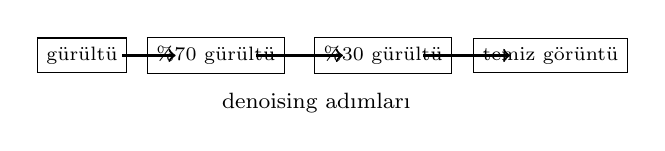
\begin{tikzpicture}[scale=0.85]
    \node at (0,0) {\fbox{\scriptsize gürültü}};
    \node at (2,0) {\fbox{\scriptsize \%70 gürültü}};
    \node at (4.5,0) {\fbox{\scriptsize \%30 gürültü}};
    \node at (7,0) {\fbox{\scriptsize temiz görüntü}};
    \draw[->,thick] (0.6,0) -- (1.4,0);
    \draw[->,thick] (2.6,0) -- (3.9,0);
    \draw[->,thick] (5.1,0) -- (6.4,0);
    \node[below=0.3em] at (3.5,-0.3) {\footnotesize denoising adımları};
  \end{tikzpicture}
  \end{center}

  \vspace{0.4em}
  \textbf{Peki metinde?} Token \emph{ayrık} (kelime), gürültü \emph{sürekli}.
  Köprü: token'ları sayı vektörlerine (embedding) çevir, gürültüyü
  oraya ekle.
\end{frame}

%==============================================================================
\begin{frame}{Diffusion-LM --- adım adım}
  \begin{enumerate}
    \item \textbf{Embed:} ``Blue Spice is a coffee shop'' kelimeleri vektörlere
          dönüşür: $x_0 \in \mathbb{R}^{L \times 768}$
    \item \textbf{Gürültüle:} her zaman adımı $t$'de farklı miktarda Gauss
          gürültüsü ekle:
          $x_t = \sqrt{\bar\alpha_t}\, x_0 + \sqrt{1-\bar\alpha_t}\, \epsilon$
    \item \textbf{Denoise:} Transformer ağı $x_t, t$'den temiz $x_0$'ı
          tahmin etmeyi öğrensin
    \item \textbf{Rounding:} tahmin edilen vektörü en yakın kelime vektörüne
          yuvarla, token'a geri dön
  \end{enumerate}

  \vspace{0.4em}
  \textbf{Eğitimde:} her batch'te rastgele bir $t$ seç, gürültüle, ağa
  ``$x_0$'ı tahmin et'' dersini ver. \\[0.3em]
  \textbf{Örneklemede:} $x_T$ = saf gürültü, 200 DDIM adımı boyunca yavaş
  yavaş temizle.
\end{frame}

%==============================================================================
\section{Yöntem: Prefix conditioning}

\begin{frame}{Prefix conditioning --- ``cümlenin başını ben yazıyorum''}
  \textbf{Fikir:} Cümlenin ilk 32 pozisyonunu \emph{MR'a} ayır, hiç gürültüleme.
  \vspace{0.3em}
  \begin{itemize}
    \item Eğitimde prefix temiz kalır, kayba dahil edilmez
    \item Örneklemede her adımda prefix tekrar MR'a sabitlenir
    \item Sonuç: model MR'dan \emph{yapısal olarak} sapamaz
  \end{itemize}

  \vspace{0.4em}
  \begin{center}
  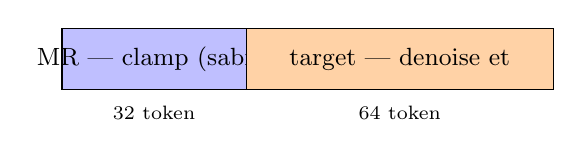
\begin{tikzpicture}[scale=0.78]
    \draw[fill=blue!25] (0,0) rectangle (3,1);
    \node at (1.5,0.5) {\small MR --- clamp (sabit)};
    \draw[fill=orange!35] (3,0) rectangle (8,1);
    \node at (5.5,0.5) {\small target --- denoise et};
    \node[below] at (1.5,-0.1) {\scriptsize 32 token};
    \node[below] at (5.5,-0.1) {\scriptsize 64 token};
  \end{tikzpicture}
  \end{center}

  \vspace{0.4em}
  \textbf{Görüntü diffusion analogu:} \emph{inpainting} ---
  resmin bir kısmını sabit tutup geri kalanını üretmek.
\end{frame}

%==============================================================================
\section{Geliştirme yolculuğu}

\begin{frame}{Geliştirirken neyle uğraştım? (1/3) --- bozuk sampler}
  \textbf{İlk çalışan versiyon:} Diffusion-LM eğitildi, BLEU \(\approx 0\),
  çıktılar tamamen kelime salatası.

  \begin{exampleblock}{Bozuk çıktı örneği}
    \footnotesize
    ``edwin with are river groveyear aired would sexes co cuisine would
    confluence participation youoga ssive establishment yourano crown and
    on prices...''
  \end{exampleblock}

  \vspace{0.3em}
  \textbf{Sorun ne?} Sampler her adımda
  $x \leftarrow \hat x_0$ yapıyordu --- diffusion'un \emph{trajectory}'sini
  takip etmiyordu, sadece tahmini yazıyordu.

  \vspace{0.3em}
  \textbf{Çözüm:} DDIM ters güncelleme:
  \[
    x_{t-1} = \sqrt{\bar\alpha_{t-1}}\, \hat x_0
            + \sqrt{1 - \bar\alpha_{t-1}}\, \hat\epsilon
  \]
  \textbf{Etki:} İlk anlamlı kelimeler ilk defa çıktı.
\end{frame}

%==============================================================================
\begin{frame}{Geliştirirken neyle uğraştım? (2/3) --- padding ve embedding}
  \textbf{Sorun A: padding'i de ``denoise'' ediyordu}
  \begin{itemize}
    \item Hedef 64 token'a göre boyutlanmış, çoğu padded
    \item Model kapasitesini boşluk modellemeye harcıyordu
    \item \textbf{Çözüm:} \texttt{target\_mask} ile MSE ve CE kaybını sadece
          gerçek hedef pozisyonlarda hesapla
  \end{itemize}

  \vspace{0.5em}
  \textbf{Sorun B: rastgele embedding'ler çöküyordu}
  \begin{itemize}
    \item Embedding tablosu rastgele başlatılınca tüm token'lar yakın
          vektörlere çöküyor
    \item Rounding (en yakın token) anlamsız sonuçlar veriyor
    \item \textbf{Çözüm:} embedding tablosunu \texttt{bert-base-uncased}
          embedding'leriyle başlat --- meaningful geometry hediye
    \item \textbf{Etki:} \emph{tek değişikliğin en büyük kalite sıçraması}
  \end{itemize}
\end{frame}

%==============================================================================
\begin{frame}{Geliştirirken neyle uğraştım? (3/3) --- iyileştirmeler}
  Daha sonra üç ``modern'' diffusion tekniğini ekledim:
  \vspace{0.3em}

  \textbf{1. Self-conditioning} (Chen et al.\ 2022)
  \begin{itemize}
    \item Denoiser önceki $\hat x_0$ tahminini de girdi alır
    \item Adımlar arası bilgi paylaşımı --- küçük model için kritik
  \end{itemize}

  \textbf{2. EMA ağırlıkları} (Ho et al.\ 2020)
  \begin{itemize}
    \item Eğitim ağırlıklarının yavaş hareketli ortalaması
    \item Epoch'tan epoch'a örnek kalitesi varyansı düştü
  \end{itemize}

  \textbf{3. Classifier guidance} (Dhariwal \& Nichol 2021)
  \begin{itemize}
    \item Ortak eğitilen ``food sınıflandırıcısı''
    \item Örneklemede gradient ile hedef yemek tipine doğru itme
    \item \emph{Yumuşak kontrol}: prefix clamping'in tamamlayıcısı
  \end{itemize}
\end{frame}

%==============================================================================
\begin{frame}{İki kontrol mekanizması --- sert ve yumuşak}
  \begin{columns}[T]
    \column{0.5\textwidth}
    \textbf{Sert: prefix clamping}
    \begin{itemize}
      \item MR hiç değişmez, hiç gürültülenmez
      \item ``Blue Spice'' adı çıktıda olmak zorunda
      \item Yapısal olarak garantili
      \item Esneklik yok
    \end{itemize}

    \column{0.5\textwidth}
    \textbf{Yumuşak: classifier guidance}
    \begin{itemize}
      \item Gradient ile yönlendirme
      \item ``Italian'' $\to$ ``Italian cuisine'' paraphrase serbest
      \item Akıcılık $\leftrightarrow$ kontrol takası
      \item Esnek
    \end{itemize}
  \end{columns}

  \vspace{0.8em}
  \begin{alertblock}{Tasarım kararı}
    İkisini birlikte kullandım: \emph{verbatim} olması gereken slotlar
    (\texttt{name}) için sert; \emph{paraphrase} olabilecek slotlar
    (\texttt{food}) için yumuşak.
  \end{alertblock}
\end{frame}

%==============================================================================
\section{Karşılaştırma ve değerlendirme}

\begin{frame}{Karşılaştırdığım baseline'lar}
  \begin{block}{GPT-2 small (otoregresif decoder)}
    \begin{itemize}
      \item ``\texttt{MR <|sep|> referans}'' formatıyla fine-tune
      \item \textbf{Nucleus sampling} ($p=0.95$) --- en çeşitli çıktı
    \end{itemize}
  \end{block}

  \begin{block}{T5-small (encoder-decoder)}
    \begin{itemize}
      \item Source = MR, Target = referans
      \item \textbf{Beam search} (b=4) --- en yüksek akıcılık
    \end{itemize}
  \end{block}

  \begin{block}{Diffusion-LM (önerilen)}
    \begin{itemize}
      \item Yukarıda anlattığım tüm geliştirmelerle
      \item 6 katman, 8 head, hidden 512, 20 epoch (A100)
    \end{itemize}
  \end{block}

  \textbf{Ölçtüğüm üç eksen:} akıcılık (BLEU, ROUGE-L), çeşitlilik
  (distinct-1/2), kontrol (slot accuracy).
\end{frame}

%==============================================================================
\begin{frame}{Ana sonuçlar --- E2E NLG test seti (4{,}693 örnek)}
  \begin{table}
    \centering
    \renewcommand{\arraystretch}{1.25}
    \begin{tabular}{lccccc}
      \toprule
      Model & BLEU & ROUGE-L & dist-1 & dist-2 & Slot Acc. \\
      \midrule
      GPT-2 (nucleus)       & \dots & \dots & \dots & \dots & \dots \\
      T5-small (beam-4)     & \dots & \dots & \dots & \dots & \dots \\
      \textbf{Diffusion-LM} & \dots & \dots & \dots & \dots & \dots \\
      \bottomrule
    \end{tabular}
  \end{table}

  \vspace{0.4em}
  \textbf{Beklenen örüntü (literatür + ablation'lar):}
  \begin{itemize}
    \item T5 + beam search: \emph{en akıcı}, ama en tekrarlı (en düşük distinct)
    \item GPT-2 + nucleus: \emph{en çeşitli}, orta akıcılık
    \item Diffusion-LM: arada bir nokta --- çeşitlilik ve kontrol dengesi
  \end{itemize}

  \vspace{0.3em}
  \footnotesize Mesaj: tek bir ``en iyi'' model yok; tasarım hedefine göre
  doğru aracı seç.
\end{frame}

%==============================================================================
\begin{frame}{Ablation --- neyi değiştirsem ne olur?}
  \begin{table}
    \centering
    \footnotesize
    \renewcommand{\arraystretch}{1.15}
    \begin{tabular}{lcccc}
      \toprule
      Varyant & BLEU & ROUGE-L & dist-2 & Slot Acc. \\
      \midrule
      sqrt schedule (varsayılan) & \dots & \dots & \dots & \dots \\
      cosine schedule            & \dots & \dots & \dots & \dots \\
      DDIM 50 adım               & \dots & \dots & \dots & \dots \\
      DDIM 100 adım              & \dots & \dots & \dots & \dots \\
      DDIM 200 adım              & \dots & \dots & \dots & \dots \\
      prefix uzunluğu 16         & \dots & \dots & \dots & \dots \\
      prefix uzunluğu 32         & \dots & \dots & \dots & \dots \\
      prefix uzunluğu 48         & \dots & \dots & \dots & \dots \\
      \bottomrule
    \end{tabular}
  \end{table}

  \textbf{Üç soru aradım}
  \begin{itemize}
    \item Gürültü programı (sqrt vs cosine) ne kadar fark eder?
    \item Daha az DDIM adımı $\to$ daha hızlı, ama akıcılık ne kadar düşer?
    \item Prefix kısalınca (16) slot accuracy çöker mi?
  \end{itemize}
\end{frame}

%==============================================================================
\begin{frame}{Hata analizi --- ne yanlış gidiyor?}
  \textbf{Slot bazında failure modes}
  \begin{itemize}
    \item \texttt{food}, \texttt{near} en yüksek miss oranı (geniş vokabüler)
    \item T5 verbatim'da en sadık ama \emph{template'e kilitleniyor}
    \item GPT-2 çelişkili MR'ları (high price + low rating) hedge ile
          ``halüsine'' ediyor
    \item Diffusion-LM + classifier guidance: \texttt{food} accuracy'sini
          spesifik olarak yukarı çekiyor
  \end{itemize}

  \vspace{0.6em}
  \textbf{Guidance scale taraması}
  \begin{itemize}
    \item $s > 1.0$: slot accuracy ↑, ama BLEU ↓ (manifold'dan kayma)
    \item $s < 0.2$: yönlendirme yok gibi
    \item Seçim: $s = 0.5$ --- ``elbow'' noktası
  \end{itemize}
\end{frame}

%==============================================================================
\section{Sonuç ve öğrendiklerim}

\begin{frame}{Ne öğrendim?}
  \begin{block}{Teknik dersler}
    \begin{itemize}
      \item \textbf{Diffusion metinde zorlu} --- görüntüden çok daha az
            ``forgiving''; padding mask gibi küçük detaylar belirleyici
      \item \textbf{Pretrained embedding init} en büyük tek-değişiklik
            etkisini yapar
      \item Sert + yumuşak kontrolün \emph{birlikte} kullanımı en pratik
            tasarım kararı
    \end{itemize}
  \end{block}

  \begin{block}{Daha geniş ders}
    \begin{itemize}
      \item ``Yeni paradigma'' her zaman ``daha iyi'' demek değil ---
            AR baseline'lar şaşırtıcı derecede güçlü
      \item Doğru ölçüm metriği görev kadar önemli (slot-fill permissive bir
            metrik; daha iyisi parser-tabanlı olur)
      \item Küçük modelle çalışırken \emph{her bir} pretrained sinyali
            kullanmak gerekiyor
    \end{itemize}
  \end{block}
\end{frame}

%==============================================================================
\begin{frame}{Gelecek çalışma}
  \begin{itemize}
    \item \textbf{Çok-başlı sınıflandırıcı:} 8 E2E slot'unu eş zamanlı
          yönlendir
    \item \textbf{Parser-tabanlı slot metriği:} çıktıyı parse edip MR'a geri
          dön, slot-bazında compare et
    \item \textbf{Daha açık vokabüler:} CommonGen gibi benchmark'ta dene
    \item \textbf{Daha büyük denoiser:} 6 katman $\to$ 12+ katman, ölçek
          etkisini görme
    \item \textbf{Cross-attention prefix:} clamp yerine learned cross-attn
          ile MR enjeksiyonu
  \end{itemize}
\end{frame}

%==============================================================================
\begin{frame}{Özet}
  \begin{block}{Yaptığım iş}
    \begin{enumerate}
      \item Diffusion-LM'i sıfırdan implemente ettim (E2E NLG için
            prefix-koşullu varyant)
      \item Eğitim sırasında birkaç bug'ı tespit edip düzelttim
            (sampler, mask, embedding init)
      \item Üç modern tekniği ekledim: self-conditioning, EMA,
            classifier guidance
      \item GPT-2 ve T5 ile üç eksenli karşılaştırma + üç ablation ekseni
    \end{enumerate}
  \end{block}

  \begin{exampleblock}{Götürdüğüm cümle}
    Diffusion-tabanlı metin üretimi \emph{çeşitlilik--kontrol} dengesinde
    AR modellere alternatif olabiliyor; \emph{saf akıcılıkta} hâlâ
    T5 + beam search önde, ama iki kontrol mekanizmasını
    (sert + yumuşak) birleştirebilmek pratik bir avantaj.
  \end{exampleblock}
\end{frame}

%==============================================================================
\begin{frame}{Kaynaklar (seçilmiş)}
  \footnotesize
  \begin{thebibliography}{9}
    \bibitem{li2022} Li, X.L., Thickstun, J., Gulrajani, I., Liang, P., Hashimoto, T.B.
      \newblock Diffusion-LM Improves Controllable Text Generation. \emph{NeurIPS}, 2022.
    \bibitem{ho2020} Ho, J., Jain, A., Abbeel, P.
      \newblock Denoising Diffusion Probabilistic Models. \emph{NeurIPS}, 2020.
    \bibitem{song2021} Song, J., Meng, C., Ermon, S.
      \newblock Denoising Diffusion Implicit Models. \emph{ICLR}, 2021.
    \bibitem{dhariwal2021} Dhariwal, P., Nichol, A.Q.
      \newblock Diffusion Models Beat GANs on Image Synthesis. \emph{NeurIPS}, 2021.
    \bibitem{chen2022} Chen, T., Zhang, R., Hinton, G.
      \newblock Analog Bits: Generating Discrete Data Using Diffusion Models with
      Self-Conditioning. \emph{arXiv:2208.04202}, 2022.
    \bibitem{novikova2017} Novikova, J., Dušek, O., Rieser, V.
      \newblock The E2E Dataset: New Challenges for End-to-End Generation.
      \emph{SIGDIAL}, 2017.
    \bibitem{dusek2019} Dušek, O., Howcroft, D.M., Rieser, V.
      \newblock Semantic Noise Matters for Neural Natural Language Generation.
      \emph{INLG}, 2019.
  \end{thebibliography}
\end{frame}

%==============================================================================
\begin{frame}[plain]
  \centering
  \vspace{2em}
  {\Huge \textbf{Teşekkürler}}
  \vspace{1.5em}

  {\Large Sorular?}
  \vspace{2em}

  \footnotesize
  Zübeyr Almaho \quad|\quad 300201023 \\
  \texttt{zubeyralmaho@std.iyte.edu.tr} \\
  \vspace{0.4em}
  \texttt{github.com/zubeyralmaho/diffusion-lm-ctg}
\end{frame}

\end{document}
